\chapter{Conclusions}
\label{ch:conclusions}

This thesis continued the work presented in \cite{Calabrese2017}, completing the design and implementation of a high-speed SS-OCT system. An axial resolution of $\sim 11$ $\mu$m was achieved in air,  comparable to the theoretical value of $\sim9$ $\mu$m. Using a resolution test target the lateral resolution was also experimentally determined, reaching values as low as $\sim 14$ $\mu$m and thus providing a substantial improvement on the $22$ $\mu$m predicted by theory. \\

\noindent A multi-processing C++ OCT software capable of real-time low-delay video performance was entirely developed, integrating the control of the galvanometric mirrors and the high speed data acquisition board. Using this system, a wide range of samples have been imaged, producing axial, cross-sectional and volumetric data. Additionally, two methods to obtain \emph{en-face} projections from three-dimensional data have been compared. Finally, a basic OpenGL volume rendering and slicing application has been implemented. \\


\begin{figure}[htb]
	\myfloatalign
	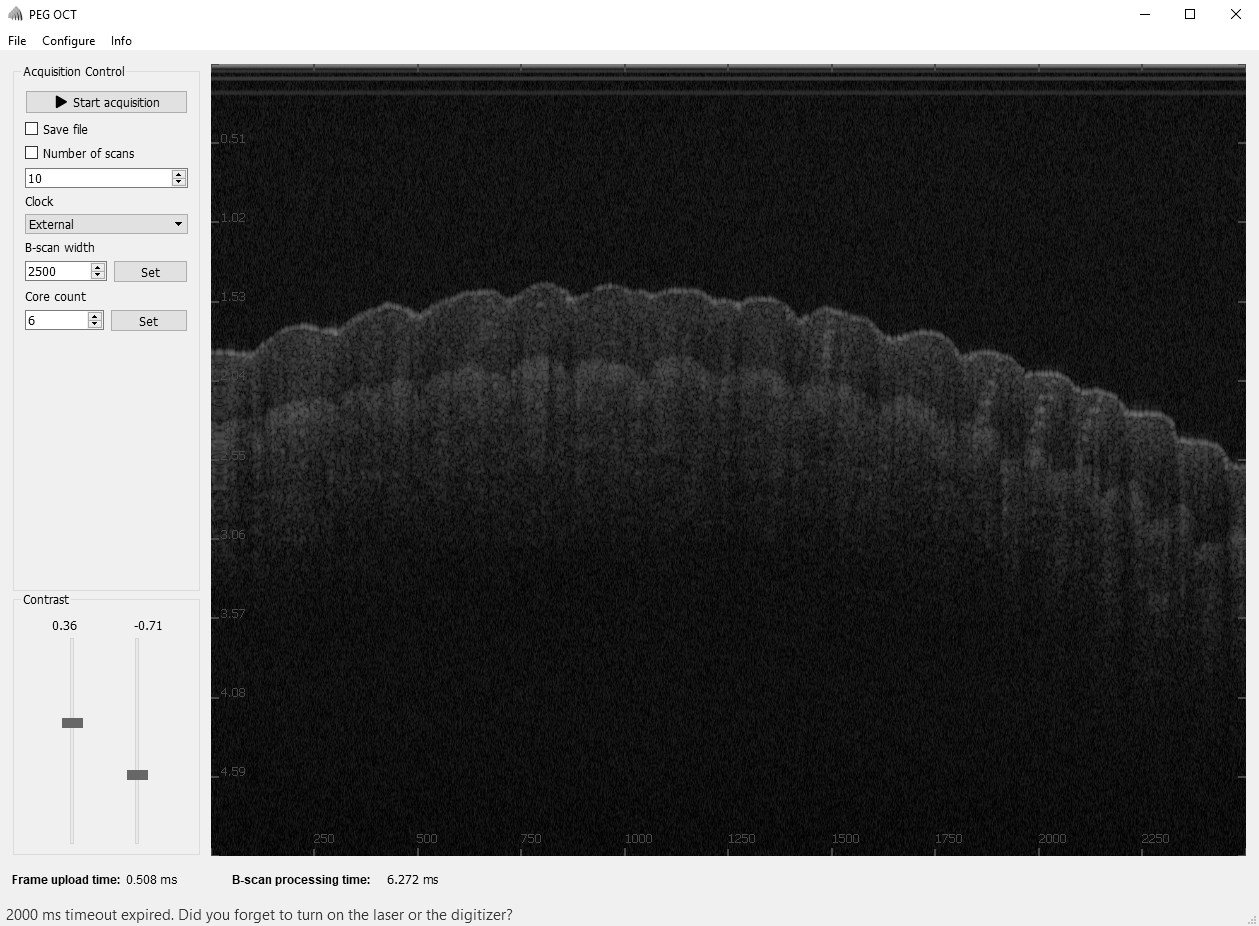
\includegraphics[width=1\linewidth]{gfx/ch4/gui}
	\caption{The \ac{GUI} of the final OCT application, showing a B-scan of a finger.}\label{fig:gui}
\end{figure}


\noindent Future developments of this work include the design of a polarization sensitive SS-OCT scheme capable of birefringence measurements, along with the migration of the FFT computation from the FPGA module integrated on the DAQ board to the GPU, using a GPGPU approach. Several other improvements can be made, including the use of photodiodes designed to work in the 1310 nm range and the design of a dispersion compensating technique to enhance the axial resolution of the system. More advanced and efficient volume rendering algorithms can also be implemented to facilitate the visualization of 3D data. 


